\chapter{Code Obfuscation}

Code Obfuscation is a technique by which programmers have deliberately sought to make the functionality of their code less obvious. This technique has been used by programmers to achieve various additional objectives.

Some of the advantages of code obfuscation, that make it very popular amongst software developers are:

\begin{itemize}
	\item Prevention of reverse engineering.
	\item Protection of intellectual property.
	\item Reducing the size of an executable.
	\item Protection of licensing mechanisms.
	\item Restricting unauthorized access.
\end{itemize}


We will look at the history of code obfuscation to appreciate the relevance of code obfuscation in today's software development perspective.

\section{Growth of Obfuscation in Software Development}

Code obfuscation has been historically associated with malware development, than with benign software development. Some of the earliest examples of attempts at obfuscation in malware can be found in the \"Brain Virus" \cite{brain} . In this variant of the malware, the malicious program would display unaffected disk partitions to users attempting to access partitions that the virus had corrupted. Although the code in itself was not encrypted, the behavior of the virus shows attempts at hiding its true usage.

In the same year, the Cascade virus was released to the world. This was an early variant of malware to use encryption to hide its true purpose. The earliest strains of obfuscated malware used a simple encryption-decryption routine to perform the decryption tasks. As the malware detectors of the time were not sophisticated enough to detect the encrypted part of the code, this simple obfuscation technique enabled a lot of malware programs to slip away undetected. This is a serious disadvantage in the design and implementation of malware detectors. We would be exploring more such flaws with the implementation of malware detectors in this project.

With the advent of advanced malware detectors and improvement in statical analysis techniques, the level of obfuscation in malware increased. Polymorphic malware uses a very high level of encryption technique to obfuscate its contents. A polymorphic malware changes the encryption in itself and provides very few traces of a signature. If a malware is truly polymorphic, then there will be no consistency between any two iterations of the same program and it would be virtually impossible to detect them using traditional signature matching techniques.

\section{Malware Detectors}

Malware detectors came into existence with the advent of different malicious programs. Before the rapid growth of the internet, malware detectors were only capable of performing scans based on signatures of known virus programs. This static analysis technique meant that new virus would be out in the wild for some time before the malware definitions of the individual anti virus programs could be updated.

With the introduction of the world wide web, the antivirus industry expanded into dynamic analysis and cloud based malware detectors. Firewalls, online scanning, and virtual machines started being increasingly used to identify malware. One major shortfall of anti virus programs is their inability to detect polymorphic virus. The various methods employed by antivirus programs include:

\begin{enumerate}
	\item Signature Based Detection
	\item Heuristics Based Detection
	\item Rootkit Detection
	\item On-Access Scanning	
\end{enumerate}

The functioning of theses methods, their limitations, and their relevance to this experiment are discussed in the next few pages.

\subsection{Signature Based Detection}
	This is one of the most basic methods of malware detection that is still in use today. When a new strain of malware is detected in the "wild", antivirus firms analyze it and extract a "signature" from it. This signature extraction can either be done manually or by using automated signature detection techniques \cite{ask}. Once a signature is detected, it is updated into various malware definitions of antivirus software.
	
	Although this method is effective against generic malware, it is highly ineffective against oligomorphic, polymorphic and metamorphic malware. These are variants of malware that encrypt itself with each iteration. In this project, we attempt to identify the various factors that contribute to malware detection and their importance in overcoming the signature detection method.

\subsection{Heuristics Based Detection}
	In Heuristics based detection techniques, a single signature or pattern is used to detect multiple malware belonging to the same family. Such techniques rely on the fact that multiple malware are created from a single malware. Thus, successfully creating a signature for a base family will result in the detection of all malware related to that particular family.
\subsection{Rootkit Detection}
	A rootkit is a type of software that attempts to gain administrator privileges in a system without the knowledge of the user running it. In many cases, the rootkits contain software within them that becomes undetectable to antivirus programs. Rootkits usually have full administrative access and also have the ability to hide themselves from the list of running processes. Modern antivirus software scans for rootkits in specific, to detect them. It is very difficult to remove a rootkit when compared to other generic malware programs.
\subsection{On-Access Scanning}
	In this method, the antivirus program looks out for any threats that might happen on a real-time basis. The antivirus monitors the system in which it is installed and looks for suspicious activity whenever the computer's memory is loaded with fresh data from the storage disks. This might happen when a USB drive is inserted, an email attachment is opened or a even when an already existing file is opened by a user or a program.
	This type of scanning is more effective as it does not rely solely on malware definitions to detect viruses.

\section{Android Malware Detectors}
	With the rise of the Android Operating systems, the amount of malware associated with it has also risen significantly. From a market share of 2.8 \% in 2009 \cite{androidShare2009} , Android captured about 75\% of the market in 2012 \cite{androidShare2009}. As shown in fig.~\ref{osMarketShare} , we can see that the growth and adoption of Android has been very steep. This rapid proliferation of Android resulted in an equally rapid rise of Android malware.
	
	\begin{figure}[osMarketShare]
		\centering
		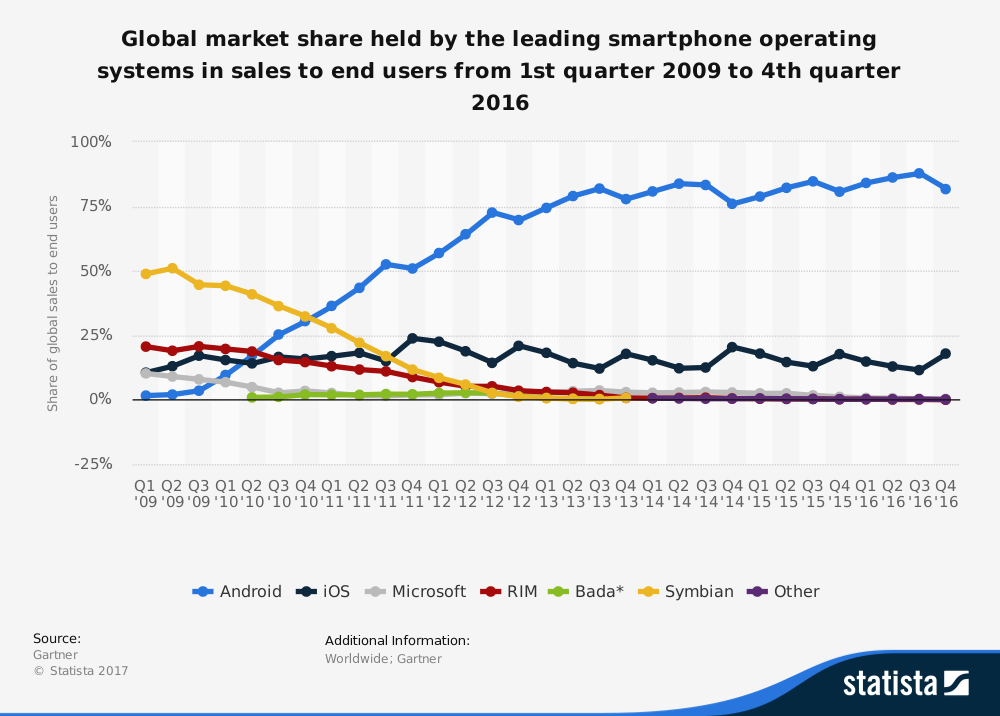
\includegraphics[width=0.5\textwidth]{OS_Market_Share.png}
		\caption{Market Share of mobile operating systems}
		\label{osMarketShare}
	\end{figure}

	With the increase in the number of Android malware being released to the wild, their level of sophistication also increased. Android malware detectors used the number of permissions requested by an app to determine its legitimacy. As shown in the fig. ~\ref{permissionsAndroid} obtained from \cite{zhou}, we can see that benign and malicious Android applications have access requests that are very similar. 	
	
	\begin{figure}[permissionsAndroid]
			\centering
			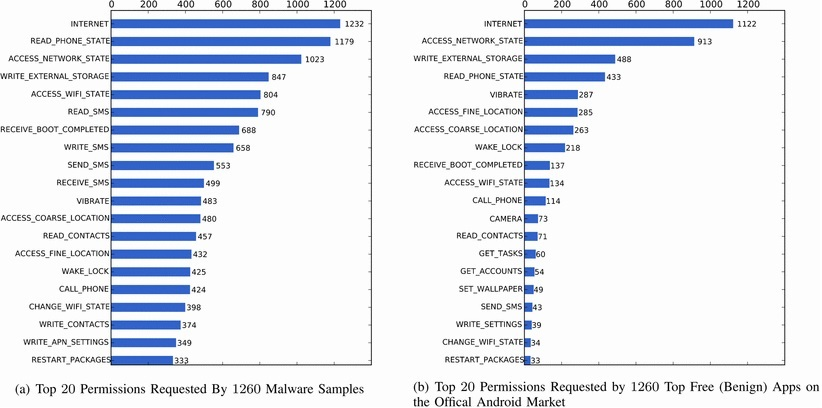
\includegraphics[width=200mm]{permissionsList.jpg}
			\caption{Top 20 permissions in Android in 2012}
			\label{permissionsAndroid}
	\end{figure}
		
	Due to this, using access requests as a measure for classifying android applications became ineffective. The various types of Android malware can be broadly classified into the following categories, depending on the type of malicious activities they perform \cite{zhou}:
	
	\begin{itemize}
		\item Privilege Escalation
		\item Remote Control
		\item Monetary Loss
		\item Information Collection
	\end{itemize}
	
	\subsection{Privilege Escalation}
		In this type of attack, the malicious app that is installed on a device, attempts to grant itself additional privileges than the one it requires. This is achieved by using known exploits in the Android operating system.
	\subsection{Remote Control}
		A very high percentage of malware attempts to use the compromised device as a remote bot. In some malware families, the remote URL that is being used to control the device. Such encryption makes it very difficult to detect these types of malware and this will be a primary area of focus in this thesis.
	\subsection{Monetary Loss}
		
	